\section{Программная реализация задачи}

\href{https://github.com/utpwtb/ITMO/tree/main/4%20%D0%92%D1%8B%D1%87%D0%B8%D1%81%D0%BB%D0%B8%D1%82%D0%B5%D0%BB%D1%8C%D0%BD%D0%B0%D1%8F%20%D0%9C%D0%B0%D1%82%D0%B5%D0%BC%D0%B0%D1%82%D0%B8%D0%BA%D0%B0/%D0%9F%D1%80%D0%BE%D0%B3%D1%80%D0%B0%D0%BC%D0%BC%D0%B0/Lab3/CM_Lab3}{{\color{blue} GitHub - Лабораторная работа №3}}

\begin{lstlisting}[style=javaStyle, label=code:gauss]

\end{lstlisting}

\section{Блок-схема реализованного алгоритма}

\begin{figure}[h]
    \centering
    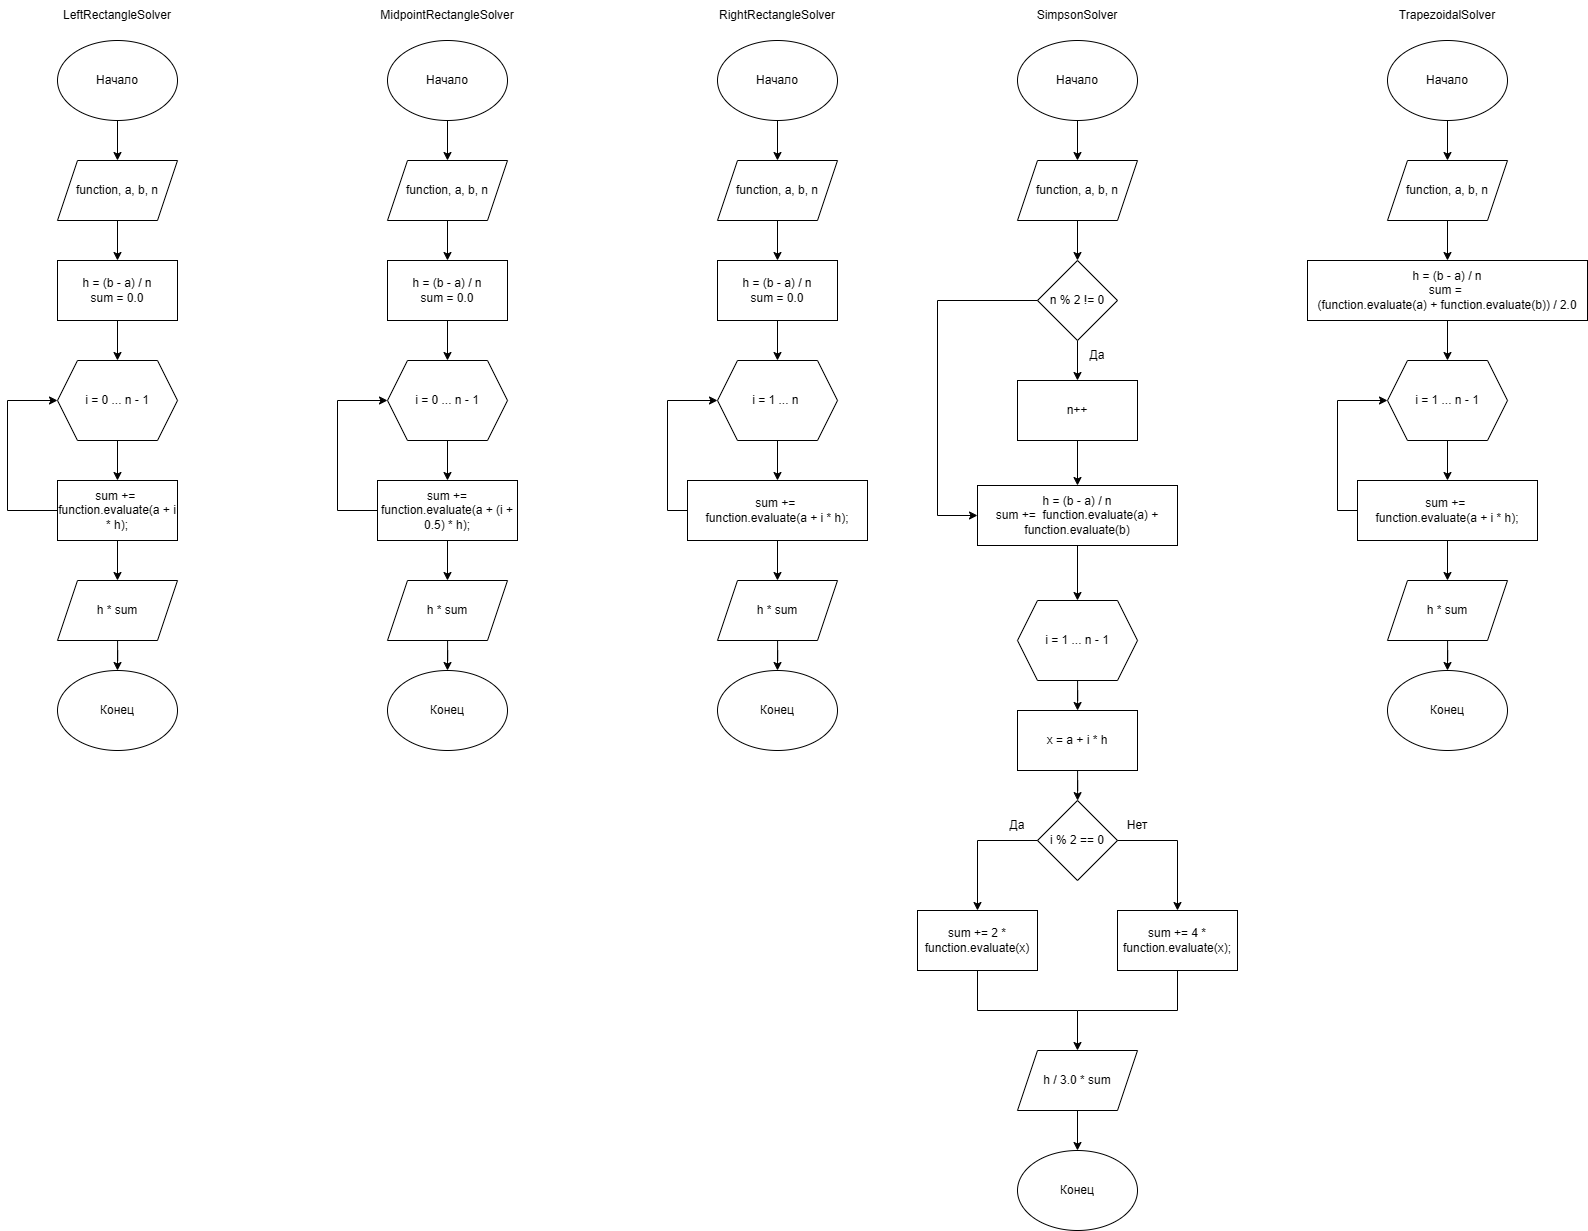
\includegraphics[width=1\linewidth]{pic/Lab3.drawio.png}
    \caption{Блок-схема}
    \label{fig:placeholder}
\end{figure}

\newpage

\section{Пример работы программы}

\begin{figure}[h]
    \centering
    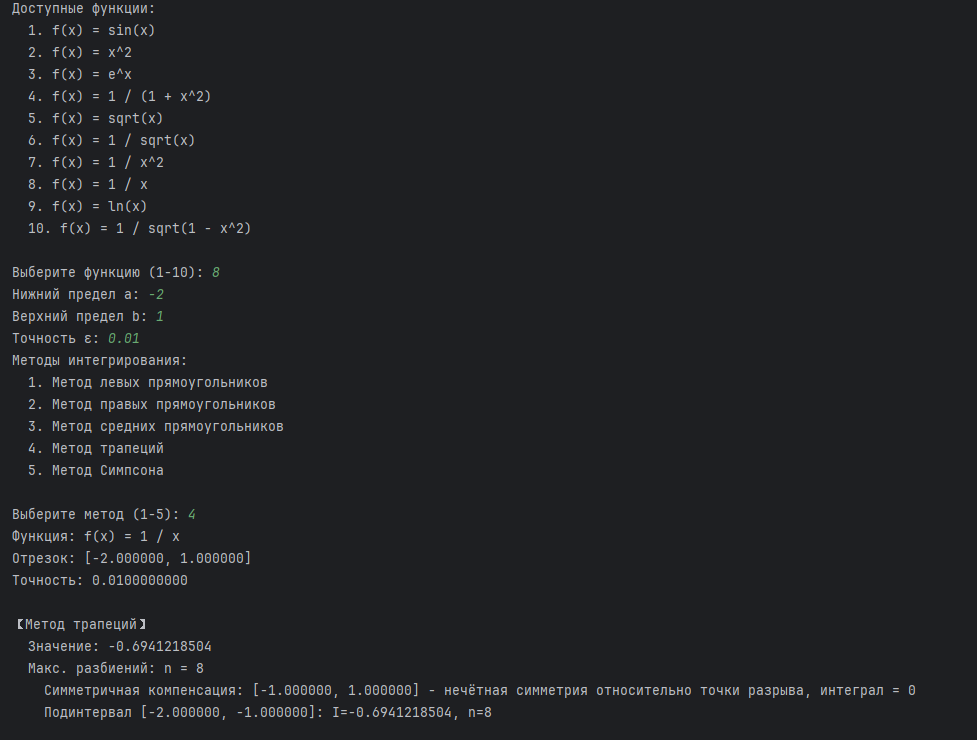
\includegraphics[width=0.5\linewidth]{pic/sp20260423_002931_949.png}
    \caption{Res 1}
    \label{fig:placeholder}
\end{figure}

\begin{figure}[h]
    \centering
    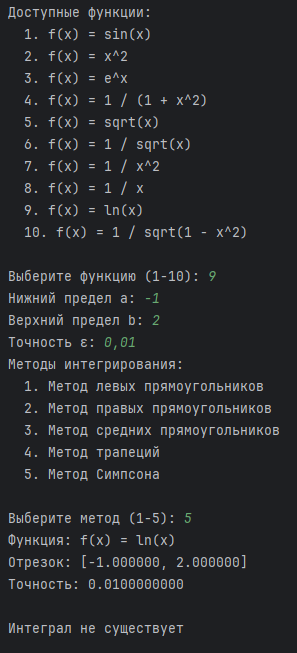
\includegraphics[width=0.25\linewidth]{pic/sp20260423_174445_952.png}
    \caption{Res 2}
    \label{fig:placeholder}
\end{figure}

\section{Вывод}

В ходе выполнения лабораторной работы были изучены численные методы интегрирования с использованием Java. В результате работы были рассмотрены различные численные методы вычисления определенных интегралов: метод прямоугольников (левых, правых, средних), метод трапеций, метод Ньютона-Котеса и метод Симпсона.
